
%(BEGIN_QUESTION)
% Copyright 2008, Tony R. Kuphaldt, released under the Creative Commons Attribution License (v 1.0)
% This means you may do almost anything with this work of mine, so long as you give me proper credit

Identifiser disse ulike ventiltypene ut fra de respektive figurene:

\vskip 10pt

\noindent
{\bf Ventil \#1:}

$$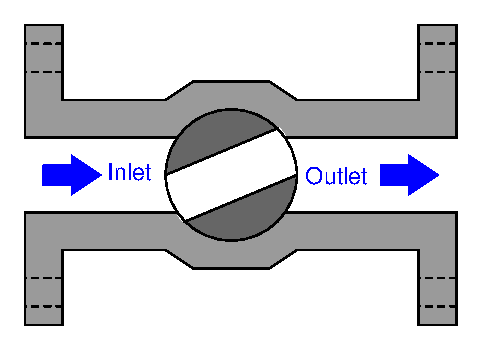
\includegraphics[width=6cm]{i00770x01.eps}$$

\vskip 10pt

\noindent
{\bf Ventil \#2:}

$$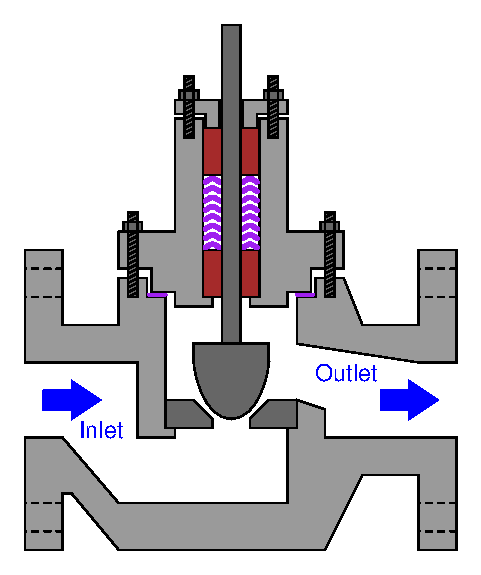
\includegraphics[width=6cm]{i00770x02.eps}$$

\vskip 10pt

\filbreak
\noindent
{\bf Ventil \#3:}

$$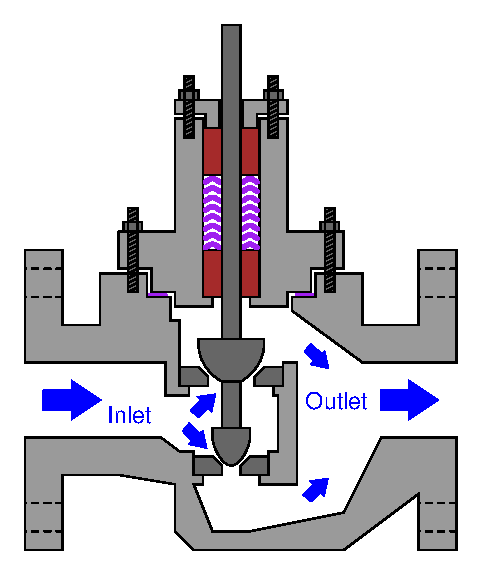
\includegraphics[width=6cm]{i00770x03.eps}$$

\vskip 10pt

\noindent
{\bf Ventil \#4:}

$$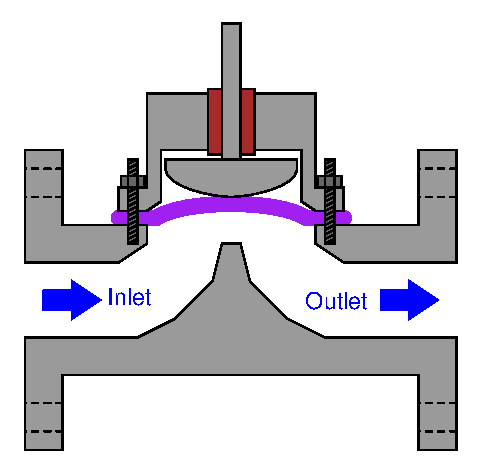
\includegraphics[width=6cm]{i00770x04.eps}$$

\vskip 10pt

\filbreak
\noindent
{\bf Ventil \#5:}

$$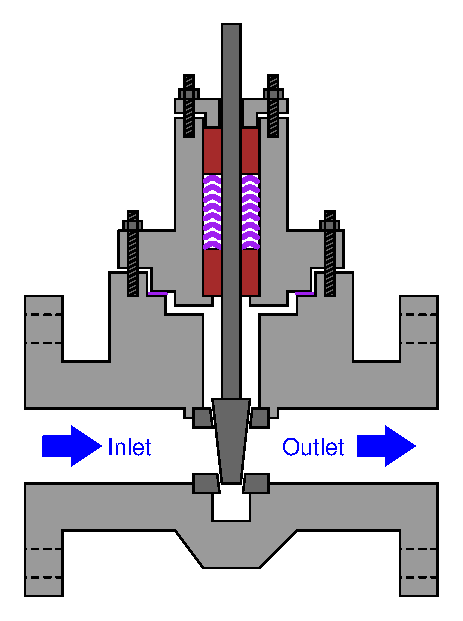
\includegraphics[width=6cm]{i00770x05.eps}$$

\noindent
{\bf Ventil \#6:}

$$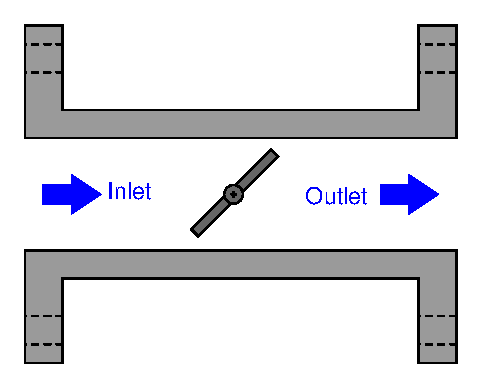
\includegraphics[width=6cm]{i00770x06.eps}$$



\underbar{file i00770}
%(END_QUESTION)





%(BEGIN_ANSWER)

Ventil \#1: Kuleventil (roterende)

\vskip 10pt

Ventil \#2: Enkeltsetet globeventil (glidende spindel)

\vskip 10pt

Ventil \#3: Dobbeltsetet globeventil (glidende spindel)

\vskip 10pt

Ventil \#4: Saunders-ventil (membran)

\vskip 10pt

Ventil \#5: Sluseventil (glidende spindel)

\vskip 10pt

Ventil \#6: Spjeldventil (roterende)

%(END_ANSWER)





%(BEGIN_NOTES)

%INDEX% Sluttkontrollelementer, ventil: typer ventilsats

%(END_NOTES)


